\chapter{Fundamental}
\label{fun}

\section{ Is there any news that drivers eth or btc}
ETH is affected by news like any other asset. News that relates to individuals trading the asset, the underlying, the development team, miners or regulation will drive the price.


Also we saw on the previous section that certain cryptocurrencies are correlated with one another so news about one could affect the other.
  
\section{ What does risk on / risk off mean?}
Risk on/ risk off refer to price responding to investor risk tolerance. During a risk on period investors have a positive sentiment about the mark so thy buy more risky assets. A risk off period is when investors have negative sentiment about the market.  During a risk off period invests will sell risky assets and buy safer assets

For example the 2008  financial crisis was a risk off period while the economic recovery in 2009 was a risk on period \cite{rri}.

\section{ How does this market react to risk on / risk off scenarios}
We will consider risk on / risk off in the terms of the covid-19 pandemic. In March when there was a lot of instability in the market people wanted to get out of their positions. Thus, we see a drop in open interest  accompanied by a massive drop in price. As the market started to recover,  investors became more risk on.  They opened more positions in crypto and price slowly increased over mid 2020. 

Figure \ref{fig:rr} illustrates the risk on and risk off periods during 2020.


\begin{figure}[H]
\center
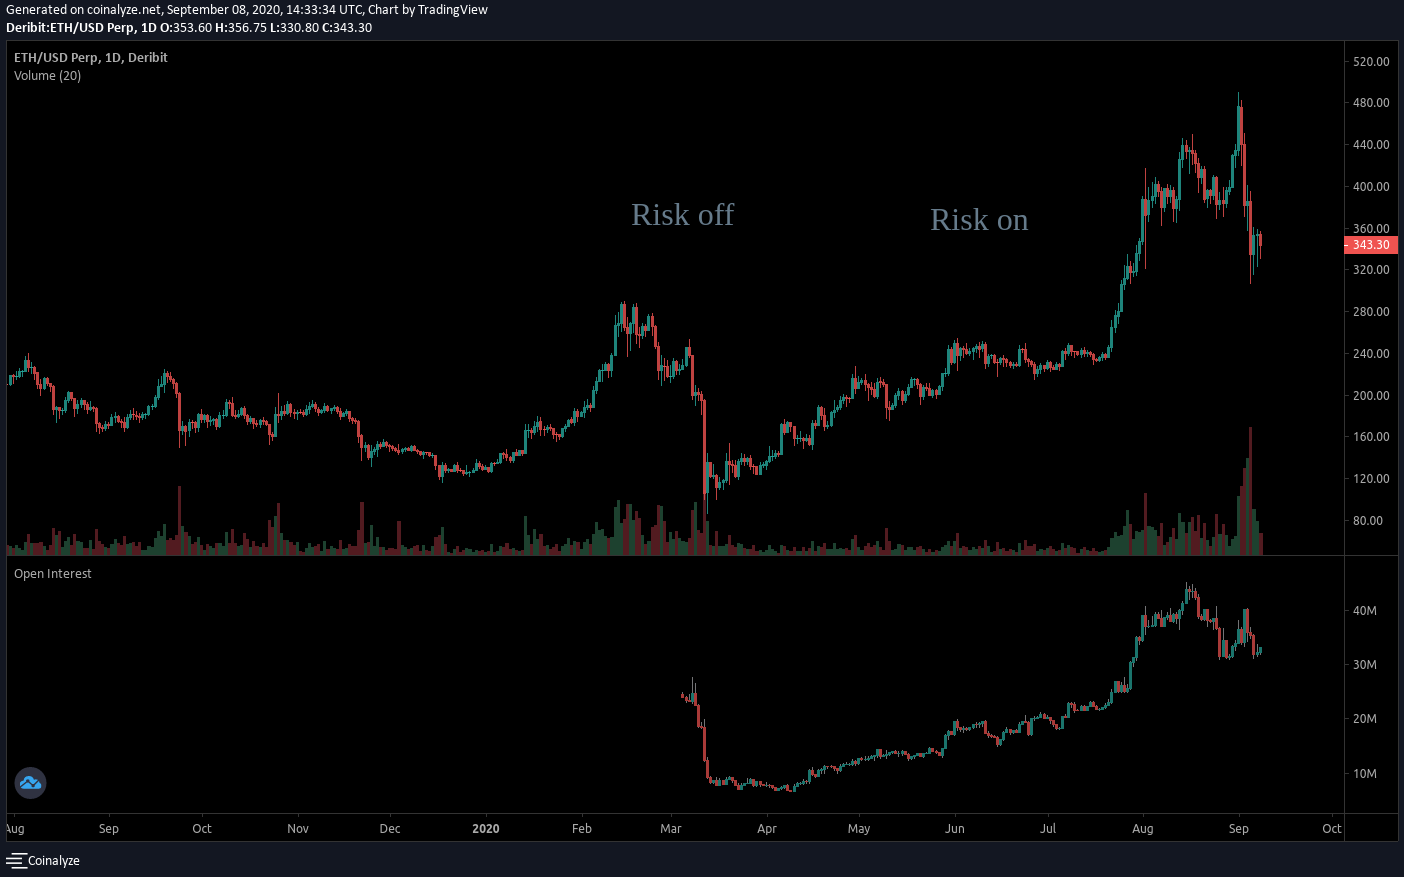
\includegraphics[width=0.9\textwidth]{fig/rr.png}
\caption{Risk on Risk off during Covid}
\label{fig:rr}
\end{figure}

\section{ Look into what caused the biggest moves (moves over $10 \%$  over the past 3 years)}
\begin{itemize}
\item Massive around Dec 2017 - In 2017 companies started to adopt the ETH infrastructure.  We also saw the emergence of many derivative tokens from these companies. Investors and tech companies amassed massive funding to further the ethereum technology.  This peaked in late 2017. In early 2018 investors took profits.
\item In early September a 30\% price drop coincided with ETH wales making large transactions
\item In late July price increased roughly 80\%.  This was in anticipation of ethereum 2.0.

\end{itemize}
\section{ When do options expire? what effect does this have?}

As of writing this report (on 9 sept 2020) we have the following option expires 

\begin{itemize}
\item 9 sept 2020
\item 10 sept 2020
\item 11 sept 2020
\item 18 sept 2020
\item 25 sept 2020
\item 30 oct 2020
\item 27 Nov 2020
\item 25 Dec 2020
\item 26 Mar 2021
\end{itemize}



\section{ What effect does this have on the market in the lead up to and the day of?}